\chapter{Introduction}
The human mouth contains several billion of bacteria living in harmony and protecting teeth from a build-up of bacteria that can harm our teeth. The unhealthy bacteria typically occur in the oral cavity after consuming food high in sugar. Dental caries results when the cariogenic bacteria build up and form a biofilm, also known as plaque. Plaque is most easily formed on rough surfaces and thus can be commonly found in fissures near the gum line and between the teeth. Bacteria composing the plaque feed on carbohydrates, and as a by-product, they produce acids, which demineralize the enamel of teeth. Teeth have a chance to remineralize if the pH of the oral cavity increases back to a regular level inadequate time and dental plaque is mechanically removed. Otherwise, caries is formed. There are different stages of dental caries progression. The early stage, when tooth decay occurs only in the enamel, can be reversed with good oral hygiene as enamel has the ability of remineralization. Once caries reach the dentine, it can not be cured and requires dental treatment to save the tooth from devitalization. Dentine does not have the ability to remineralize, hence tooth decay destroys its tissue irreversibly. The longer caries remain untreated, the more time it has to dissolve enamel and dentine causing visible cavities in the teeth. That is the reason why it is essential to make an early discovery of the illness. \\
Primary diagnosis involves inspection of visible tooth surfaces using a dentist's sight with a help of a dental mirror and a dental probe during a regularly scheduled appointment. This check-up should be arranged twice a year. In addition, it is a good practice to examine a patient's dental X-rays at least once a year since some of the caries in the early stages are difficult to be caught by eye \cite{cavityarticle}. \\
Even though the caries prevention system is highly developed, more than 3.5 billion people have been or been affected in 2017 \cite{James2018}.

Recent advances in the field of deep learning opened gates to widespread deployment in many fields, including medical science. Programs using deep learning have been able to achieve increasingly higher performance. On specialized tasks, those programs were already able to surpass human-level performance. That is a reason why  deep learning in the medical field is attracting more and more attention nowadays, causing the number of medical publications employing deep learning to increase exponentially. The amount of growth can be seen in the chart \ref{fig:med_pub} \\
The importance of dental prevention, high prevalence and incidence, and recent success of deep learning in the medical field are the motivation for this project. We will try to develop a deep learning based program, that is capable of dental caries detection from bitewing X-ray images.
\begin{figure}
    \centering
    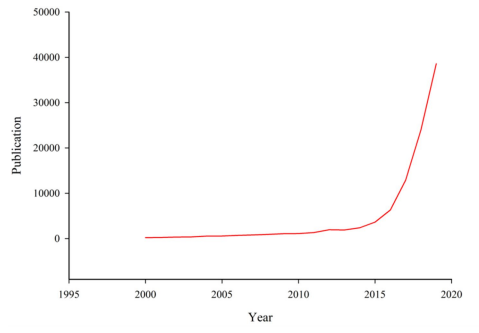
\includegraphics[width=0.7\textwidth]{images/num_publication.png}
    \caption{\label{fig:med_pub}Number of published manuscripts that uses the deep learning approach in subareas of medical health informatics \cite{Bhatt2020}}
\end{figure}